\chapter{Cubed-sphere grids}
\label{chp-cs-grids}

The cubed-sphere grid was originally proposed by \citet{sadourny:1972}
and was reinvestigated by \citet{ronchi:1996} and \citet{rancic:1996}.
As is usual to Planotic grids, we start with a Platonic solid, in this case, a cube,
circumscribed in a sphere and project its faces on the sphere.
The original cubed-sphere proposed by \citet{sadourny:1972}, called equidistant cubed-sphere, leads to non-uniform grid;
a solution to this problem was proposed with the introduction of angular coordinates, leading to a quasi-uniform grid
called equiangular cubed-sphere.
The cubed sphere then consists of six panels, each one having a local Cartesian coordinate system, which 
make it easier to extend methods from the plane to the sphere.
Indeed, \citet{putman:2007} extends the dimension splitting from \citet{lin:1996}, presented in
Chapter \ref{chp-2d-fv}, to the cubed-sphere.

	There are essentially two major challenges when working on the cubed-sphere:
1) the non-orthogonal grid system; 2) the discontinuity of the coordinate system
at the cube edges. Challenge 1) is more related to the appearance of metric terms
in the equations, which adds more computational cost requiring, for instance, several conversions
between contravariant/covariant components of a velocity field.
The second challenge, perhaps the most problematic, is related to the computation
of stencils along the cube edges, where the coordinate system is discontinuous.
A possible way to compute the stencil at the edges is to extend the local coordinate of 
each panel to its neighbor panels, adding ghost cells in the so-called halo region. 
In this case, the equiangular cubed sphere has ghost cell values, 
lying on the same geodesics containing the data from its neighbor panels,
which allows us to use one-dimensional high-order Lagrange interpolation (for a review of this method, see \citet{zerroukat:2022}).
This approach was already investing since the work of \citet{ronchi:1996}
and it is widely used in the literature \citep{Croisille:2013, katta:2015,Katta:2015b,chen:2021}.
\citet{putman:2007}, on the other hand, uses extrapolation
at grid values near the cube edges. Another approach that avoids the need for interpolation/extrapolation
near the edges is the conformal cubed-sphere developed by \citet{rancic:1996}. This grid
leads to an orthogonal and continuous coordinate system near the edges, but it generates grid singularities
near the cube corners, similar to the pole problem. An improved and more uniform conformal grid,
called Uniform Jacobian cubed sphere, was later proposed \citet{rancic:2017}.
Each approach is likely to generate grid imprinting and one of our goals
this work is to investigate how much grid-imprinting each method generates.

This chapter aims to review and investigated the geometrical properties
of the cubed-sphere. Besides that, we also aim to investigate the process
of interpolating/extrapolating near the cube edges.
We start with a basic review of the cubed-sphere mappings in Section \ref{cs-mappings},
while Section \ref{cs-halodata} investigates the interpolation/extrapolation near the cube edges
with some numerical experiments.

\section{Cubed-sphere mappings}
\label{cs-mappings}

\subsection{Equidistant cubed-sphere}
\label{equidistant-cs}

We consider a sphere radius $R>0$ and
$a = \frac{R}{\sqrt{3}}$ representing the half-length of 
the cube, and the family of maps
$\Psi_{p}: [-a,a] \times [-a,a] \to \mathbb{S}^2_R$, $p=1, \cdots, 6$,
where:
\begin{equation}
	\label{chp3-eqdistant-psi1}
	\Psi_{1}(x,y) = \frac{R}{\sqrt{a^2 + x^2 + y^2}}(a, x, y), 
\end{equation}

\begin{equation}
	\label{chp3-eqdistant-psi2}
	\Psi_{2}(x,y) = \frac{R}{\sqrt{a^2 + x^2 + y^2}}(-x, a, y), 
\end{equation}

\begin{equation}
	\label{chp3-eqdistant-psi3}
	\Psi_{3}(x,y) = \frac{R}{\sqrt{a^2 + x^2 + y^2}}(-a, -x, y), 
\end{equation}

\begin{equation}
	\label{chp3-eqdistant-psi4}
	\Psi_{4}(x,y) = \frac{R}{\sqrt{a^2 + x^2 + y^2}}(x, -a, y), 
\end{equation}

\begin{equation}
	\label{chp3-eqdistant-psi5}
	\Psi_{5}(x,y) = \frac{R}{\sqrt{a^2 + x^2 + y^2}}(-y, x, a), 
\end{equation}

\begin{equation}
	\label{chp3-eqdistant-psi6}
	\Psi_{6}(x,y) = \frac{R}{\sqrt{a^2 + x^2 + y^2}}(y, x, -a).
\end{equation}
The family of maps $\{\Psi_{p}, p = 1, \cdots, 6\}$ allow us to cover the sphere.
Here $p$ denotes a panel, and they are defined as Figure \ref{chp4-panels} shows.
\begin{figure}[!htb]
	\centering
		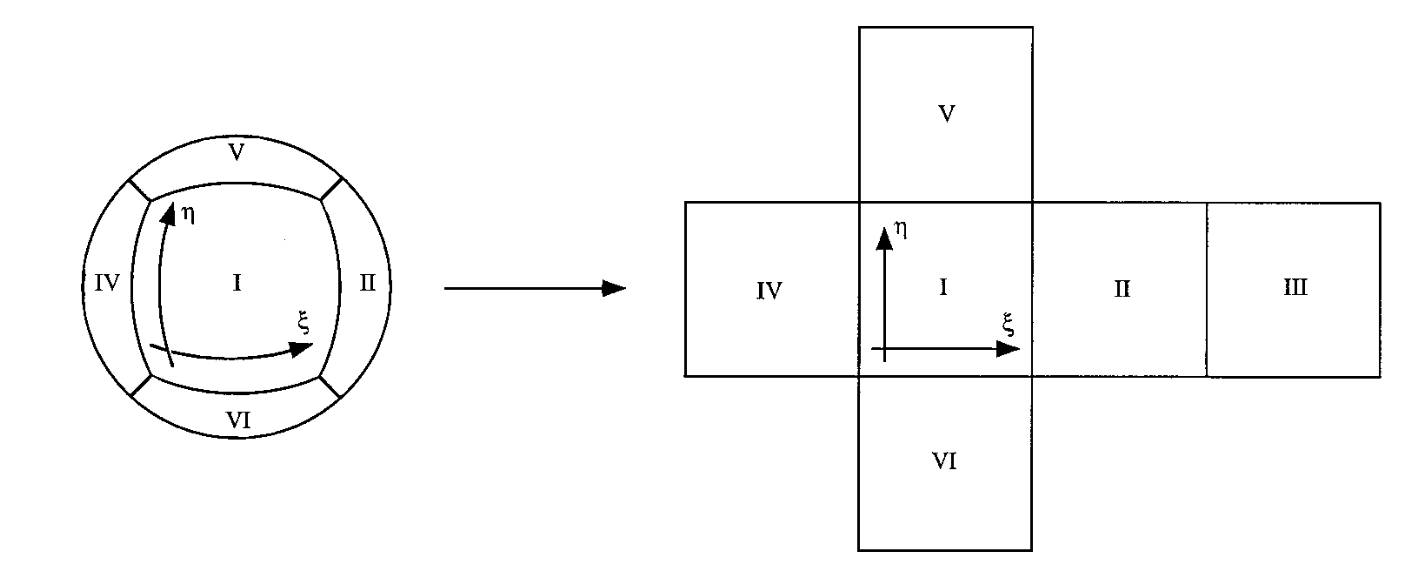
\includegraphics[width=0.8\linewidth]{chp4_panels}
	\caption{Cubed-sphere panels definition. Figure taken from \citet{ronchi:1996}.\label{chp4-panels}}
\end{figure}
The derivative of the maps $\Psi_p$ are given by:
\begin{equation}
	\label{chp3-eqdistant-dpsi1}
	D\Psi_{1}(x,y) = \frac{R}{{(a^2 + x^2 + y^2)}^{3/2}}
	\begin{bmatrix}
		-ax & -ay \\
	 	 a^2+y^2  & -xy \\
		 -xy  & a^2+x^2
	\end{bmatrix},
\end{equation}
\begin{equation}
	\label{chp3-eqdistant-dpsi2}
	D\Psi_{2}(x,y) = \frac{R}{{(a^2 + x^2 + y^2)}^{3/2}}
	\begin{bmatrix}
		-(a^2+y^2) & xy \\
		 -ax &  -ay \\
		 -xy &  a^2+x^2
	\end{bmatrix},
\end{equation}
\begin{equation}
	\label{chp3-eqdistant-dpsi3}
	D\Psi_{3}(x,y) = \frac{R}{{(a^2 + x^2 + y^2)}^{3/2}}
	\begin{bmatrix}
		 ax &  ay \\
		-(a^2+y^2) & xy \\
		 -xy &  a^2+x^2
	\end{bmatrix},
\end{equation}
\begin{equation}
	\label{chp3-eqdistant-dpsi4}
	D\Psi_{4}(x,y) = \frac{R}{{(a^2 + x^2 + y^2)}^{3/2}}	
	\begin{bmatrix}
		 a^2+y^2 &  -xy \\
		 ax & ay \\
		 -xy &  a^2+x^2
	\end{bmatrix},
\end{equation}
\begin{equation}
	\label{chp3-eqdistant-dpsi5}
	D\Psi_{5}(x,y) = \frac{R}{{(a^2 + x^2 + y^2)}^{3/2}}	
	\begin{bmatrix}
		 xy  & -(a^2+x^2) \\
	 	 a^2+y^2  &  -xy \\
		-ax & -ay
	\end{bmatrix},
\end{equation}
\begin{equation}
	\label{chp3-eqdistant-dpsi6}
	D\Psi_{6}(x,y) = \frac{R}{{(a^2 + x^2 + y^2)}^{3/2}}
	\begin{bmatrix}
		 -xy  &  a^2+x^2 \\
		 a^2+y^2  &  -xy \\
		 ax &  ay
	\end{bmatrix}.
\end{equation}
With the aid of the derivative, we may define a basis of tangent vectors 
$\{ \boldsymbol{g}_{1}, \boldsymbol{g}_{2} \}$ on each point on the sphere by:
\begin{equation}
	\boldsymbol{g}_{1}(x,y;p) = D\Psi_{p}(x,y)
	\begin{bmatrix}
		 1 \\
		 0
	\end{bmatrix},
	\boldsymbol{g}_{2}(x,y;p) = D\Psi_{p}(x,y)
	\begin{bmatrix}
		 0 \\
		 1
	\end{bmatrix}.
\end{equation}
In other words, we have $\{\boldsymbol{g}_{1}(x,y;p),\boldsymbol{g}_{2}(x,y;p)\} \subset T_{\Psi_p(x,y)}
\mathbb{S}_{R}^2$, $\forall (x,y) \in [-a,a]\times[-a,a]$ (see Appendix \ref{anexo-sph} for the definition of tangent space).
Notice that
\begin{equation}
	\label{chp3-eqdistant-psitensor}
	[D\Psi_{p}(x,y)]^TD\Psi_{p}(x,y)
	= \frac{R^2}{(a^2 + x^2 + y^2)^2}
	\begin{bmatrix}
		 a^2 + x^2 &  -xy \\
		 -xy & a^2 + y^2
	\end{bmatrix},
\end{equation}
does not depend on $p$.
Hence, it makes sense to define the matrix 
$G_{\Psi}(x,y) = [D\Psi_{p}(x,y)]^TD\Psi_{p}(x,y)$ 
which is known as metric tensor.
It is easy to see that:
\begin{equation}
	\label{chp3-eqdistant-psi-metric-tensor}
	G_{\Psi}(x,y) = 
	\begin{bmatrix}
		\langle \boldsymbol{g}_{1}(x,y;p), \boldsymbol{g}_{1}(x,y;p) \rangle & 
		\langle \boldsymbol{g}_{1}(x,y;p), \boldsymbol{g}_{2}(x,y;p) \rangle \\
		\langle \boldsymbol{g}_{1}(x,y;p), \boldsymbol{g}_{2}(x,y;p) \rangle  &
		\langle \boldsymbol{g}_{2}(x,y;p), \boldsymbol{g}_{2}(x,y;p) \rangle 
	\end{bmatrix},
\end{equation}
and that $G_{\Psi}(x,y)$ is positive-definite, 
$\forall (x,y) \in [-a,a]\times[-a,a]$.
The Jacobian of the metric tensor $G_{\Psi}(x,y)$ is then given by:
\begin{equation}
	\sqrt{|\det{G_{\Psi}(x,y)}|} = \frac{R^2}{(a^2+x^2+y^2)^{3/2}}a.
\end{equation}
\subsection{Equiangular cubed-sphere}
\label{equiangular-cs}
Another cubed-sphere mapping is the equiangular mapping \citep{ronchi:1996},
which leads to a more uniform grid. This mapping is a composition of equidistant mapping with
angular coordinates.
We consider again $a=\frac{R}{\sqrt{3}}$
and we define the family of maps
$\Phi_{p}: [-\frac{\pi}{4},\frac{\pi}{4}] 
\times [-\frac{\pi}{4},\frac{\pi}{4}] 
\to \mathbb{S}^2_R$, $p=1, \cdots, 6$,
given by $\Phi_{p}(x,y) = \Psi_{p}(a\tan{x}, a\tan{y})$.
The coordinates $(a\tan{x}, a\tan{y})$ are called angular coordinates.
By the chain rule:
\begin{equation}
	D\Phi_{p}(x,y) = a
	D\Psi_{p}(a\tan{x}, a\tan{y})
	\begin{bmatrix}
		\frac{1}{\cos^2 x} & 0 \\ 
		0 & \frac{1}{\cos^2 y} 
	\end{bmatrix},
\end{equation}
and therefore we can define the following tangent vectors
\begin{align}
	\boldsymbol{r}_{1}(x,y;p) = D\Phi_{p}(x,y)
	\begin{bmatrix}
		 1 \\
		 0
	\end{bmatrix}
	= \frac{a}{\cos^2 x}
	\boldsymbol{g}_{1}(\tan{x}, \tan{y}; p)
	,\\
	\boldsymbol{r}_{2}(x, y ;p) = D\Phi_{p}(x,y)
	\begin{bmatrix}
		 0 \\
		 1
	\end{bmatrix}
	= \frac{a}{\cos^2 y}
	\boldsymbol{g}_{2}(\tan{x}, \tan{y}; p),
\end{align}
that is, $\{\boldsymbol{r}_{1}(x,y;p),\boldsymbol{r}_{2,p}(x,y;p)\} \subset T_{\Phi_p(x,y)}
\mathbb{S}_{R}^2$, $\forall (x,y) \in 
[-\frac{\pi}{4},\frac{\pi}{4}] 
\times [-\frac{\pi}{4},\frac{\pi}{4}]$.
Again, it makes sense to define the matrix 
\begin{align}
	G_{\Phi}(x,y) &= [D\Phi_{p}(x,y)]^TD\Phi_{p}(x,y) \\
	&= a^2
	[D\Psi_{p}(a\tan{x},a\tan{y})]^T
	\begin{bmatrix}
		\frac{1}{\cos^4 x} & 0 \\ 
		0 & \frac{1}{\cos^4 y} 
	\end{bmatrix}
	D\Psi_{p}(a\tan{x}, a\tan{y}),
\end{align}
that does not depend on $p$ and is the  metric tensor.
It is easy to see that:
\begin{equation}
	\label{chp3-eqangle-phi-metric-tensor}
	G_{\Phi}(x,y) = 
	\begin{bmatrix}
		\langle \boldsymbol{r}_{1}(x,y;p), \boldsymbol{r}_{1}(x,y;p) \rangle & 
		\langle \boldsymbol{r}_{1}(x,y;p), \boldsymbol{r}_{2}(x,y;p) \rangle \\
		\langle \boldsymbol{r}_{1}(x,y;p), \boldsymbol{r}_{2}(x,y;p) \rangle  &
		\langle \boldsymbol{r}_{2}(x,y;p), \boldsymbol{r}_{2}(x,y;p) \rangle 
	\end{bmatrix},
\end{equation}
and that $G_{\Phi}(x,y)$ is positive-definite, 
$\forall (x,y) \in [-\frac{\pi}{4},\frac{\pi}{4}] 
\times [-\frac{\pi}{4},\frac{\pi}{4}]$.
The Jacobian of the metric tensor $G_{\Phi}(x,y)$ is then given by:
\begin{align}
	\label{metrictensor-cs-equiangular}
	\begin{split}
		\sqrt{|\det{G_{\Phi}(x,y)}|} &= \frac{a}{\cos^2 x \cos^2 y}
		\frac{R^2}{(a^2 + a^2\tan^2x + a^2\tan^2y)^{3/2}}a\\
		&= \frac{R^2}{\cos^2 x \cos^2 y}
		\frac{1}{(1 + \tan^2x + \tan^2y)^{3/2}}.
	\end{split}
\end{align}
Hereafter, we shall denote $g(x,y) = |\det{G_{\Phi}(x,y)}|$.
\subsection{Examples}
To represent the cubed-sphere grid, we consider the notation of Section \ref{sec:fv-2d}.
We shall assume that we have a $(\Delta x, \Delta y)-$grid of $[-a,a]^2$, with $\Delta x= \Delta y$, $N=M$,
where $a$ depends on the mapping considered.
Similarly to Chapter \ref{chp-2d-fv}, we may extend the grid to ghost cells.
Hence, for each $p=1, \cdots, 6$, we apply the mapping $\Psi_p$ or $\Phi_p$ on
each local coordinate system grid to generate the cubed-sphere with $6N^2$ cells.
In Figure \ref{chp4-cs-grid}, we depict an example of the grids generated using 
the equidistant and equiangular mappings for $N=20$.
\begin{figure}[!htb]
	\centering
	\begin{subfigure}{0.48\textwidth}
		\centering
		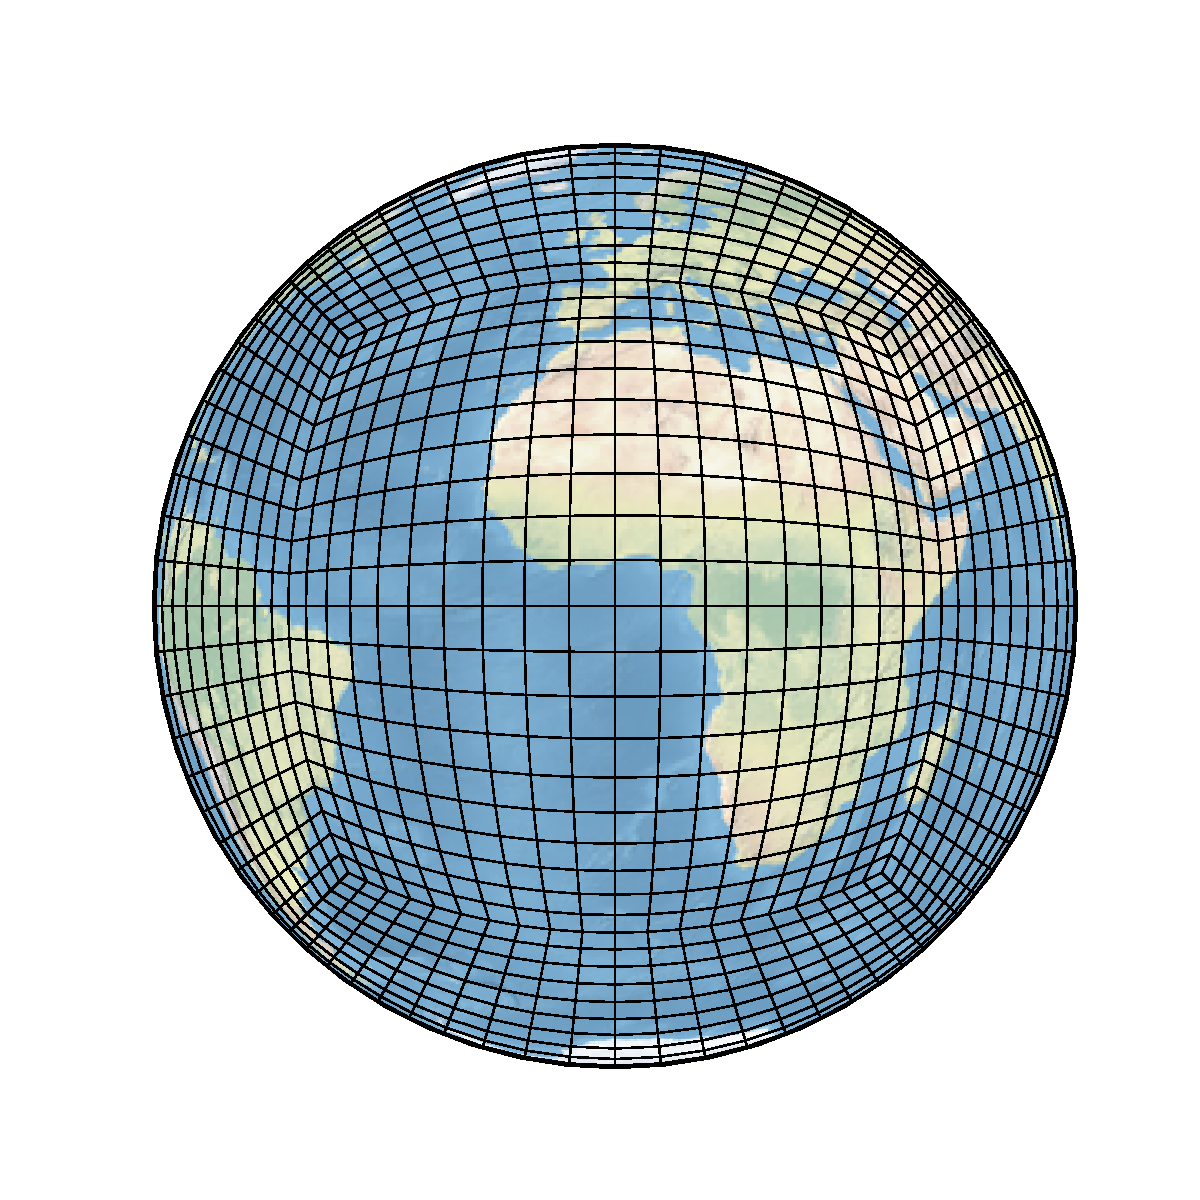
\includegraphics[width=1\linewidth]{gnomonic_equidistant_20_sphere}
		\caption{Equidistant}
	\end{subfigure}
	\begin{subfigure}{0.48\textwidth}
		\centering
		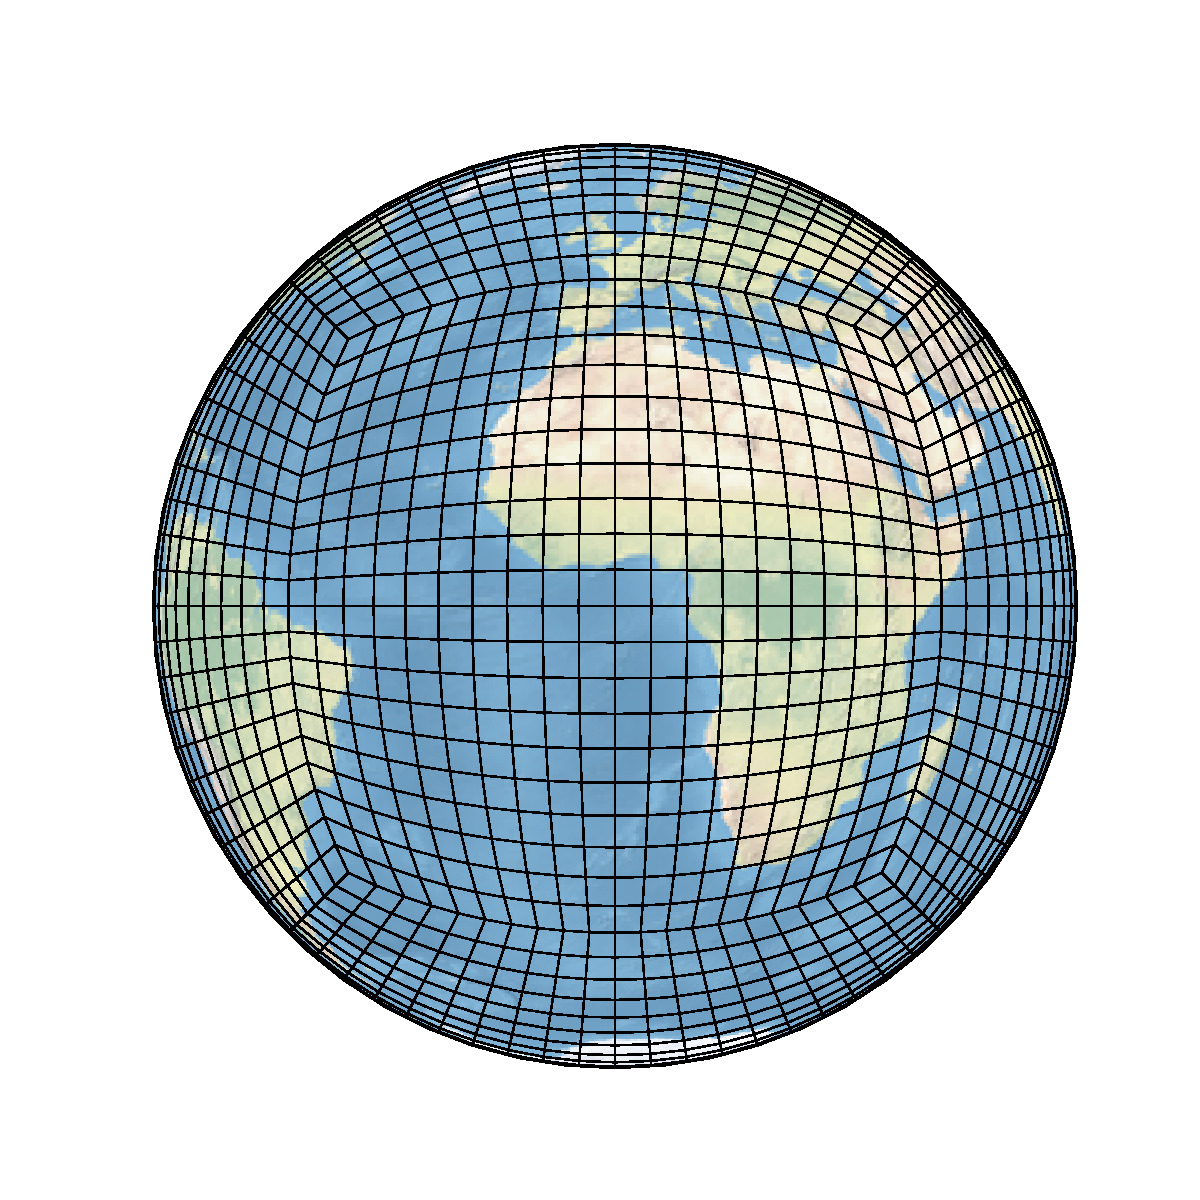
\includegraphics[width=1\linewidth]{gnomonic_equiangular_20_sphere}
		\caption{Equiangular}
	\end{subfigure}
	\caption{Equidistant (a) and equiangular (b) cubed-spheres generated with $N=20$.
		\label{chp4-cs-grid}}
\end{figure}

From Figure \ref{chp4-cs-grid}, we notice that the equiangular cubed-sphere is much more uniform
than the equidistant cubed-sphere. As pointed out by \citet{rancic:1996}, the ratio
between the maximum and minimum cell area on the equiangular cubed-sphere is approximately 1.3,
while the same ratio is approximately 5.2 on the equidistant cubed-sphere. 

\section{Edges treatment}
\label{cs-halodata}
\subsection{Ghost cells interpolation}
\label{cs-interp}
Hereafter, we are going to use the notation $(x,y;p)$ for $p=1,\cdots, 6$, to represent a
point on the sphere obtained trough the equiangular cubed-sphere mapping.
Let us assume that we have a function $q: \mathbb{S}^2_R \to \mathbb{R}$
given in the cell centroids and let us denote these values by $q_{ijp} = q(x_i,y_j;p)$,
for $i,j=1\cdots, N$, $p=1,\cdots, 6$. We wish to estimate these values outside of the range
$1, \cdots, N$, that is, we wish to estimate them at ghost cells positions.

As we pointed out before, this can be done by noticing that the ghost cells on the local
Cartesian systems are mapped onto the geodesic of a neighbor panel, which allows us to use Lagrange interpolation 
to obtain the ghost cell values.
To illustrate this process in Panel 1, in Figure \ref{chp4-cs-halodata} we depict the values of $q_{ijp}$ in Panel 1 using green circles, for $N=8$ 
and black circles for the other panels. Assuming a halo size equal to 3, we also show the target value at ghost cells 
using yellow and magenta circles. Observe that the dashed yellow lines in Figure \ref{chp4-cs-halodata} illustrate
how the ghost cells are in geodesics containing grid values from neighbor panels. Except for the magenta circles,
all the ghost values may be obtained using 1D Lagrange interpolation using the surrounding black circles on the geodesic.
This can be performed for all panels. After that, the magenta circles may be interpolated using values obtained in the first step of interpolation,
(see cyan circles in Figure \ref{chp4-cs-halodata}), preserving the order of accuracy of the interpolation, supposing this one is fixed. 
\begin{figure}[!htb]
	\centering
	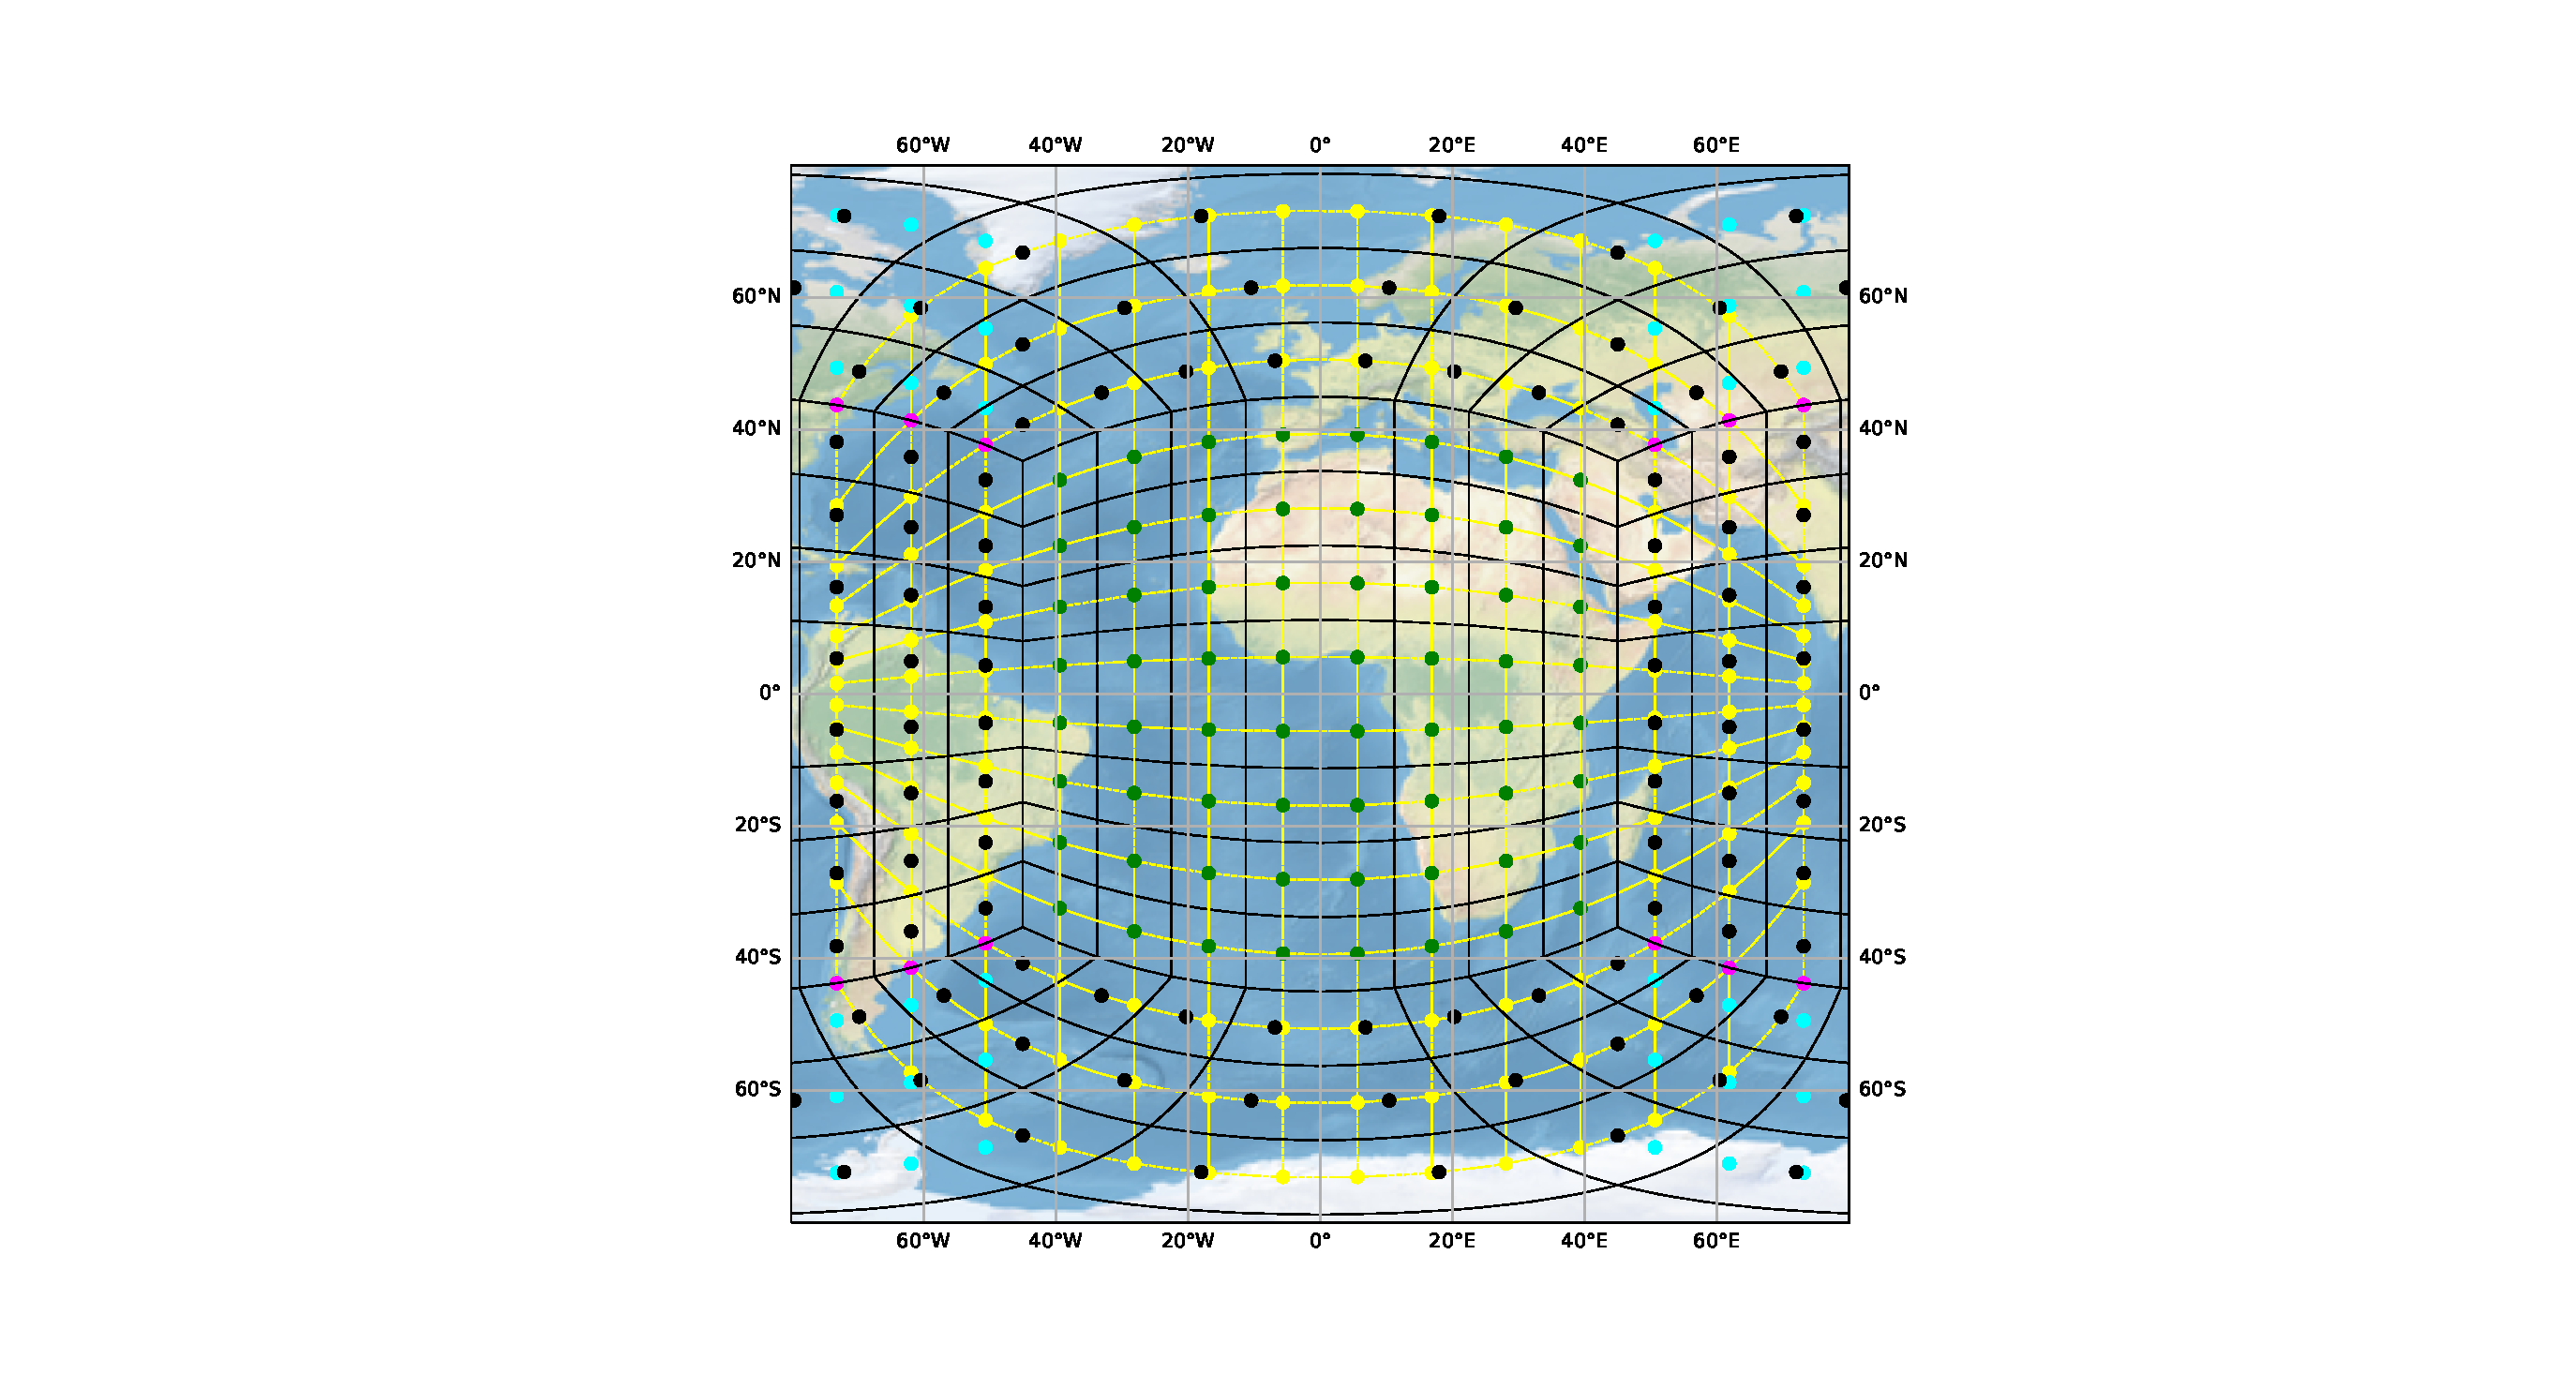
\includegraphics[width=1.0\linewidth]{gnomonic_equiangular_8_mercator}
	\caption{Equiangular cubed-sphere panel 1 with $N=8$: 
	centroid at panel 1 (green circles) and others panel centroids (black circles), 
	ghost cell points at panel 1 (yellow and magenta circles) and others panels (cyan circles).}
	\label{chp4-cs-halodata}
\end{figure}

We are going to show some numerical example of this interpolation process using a halo region of size 3 and 
assuming the radius of the sphere equal to one.
First, we consider the following function represented in $\mathbb{R}^3$ coordinates as
\begin{align}
		\label{chp4-ic1}
		q(X,Y,Z) = \exp(-10((X-X_0)^2+(Y-Y_0)^2+(Z-Z_0)^2)),
\end{align}
where $(X_0,Y_0,Z_0)$ represent the $\mathbb{R}^3$ coordinates of the latitude-longitude point
$(\frac{\pi}{4},\frac{\pi}{6})$ as in \citet{zerroukat:2022}, which consists of a Gaussian centered 
at a panel 1 corner as Figure \ref{chp4-cs-ic1} shows.
\begin{figure}[!htb]
	\centering
	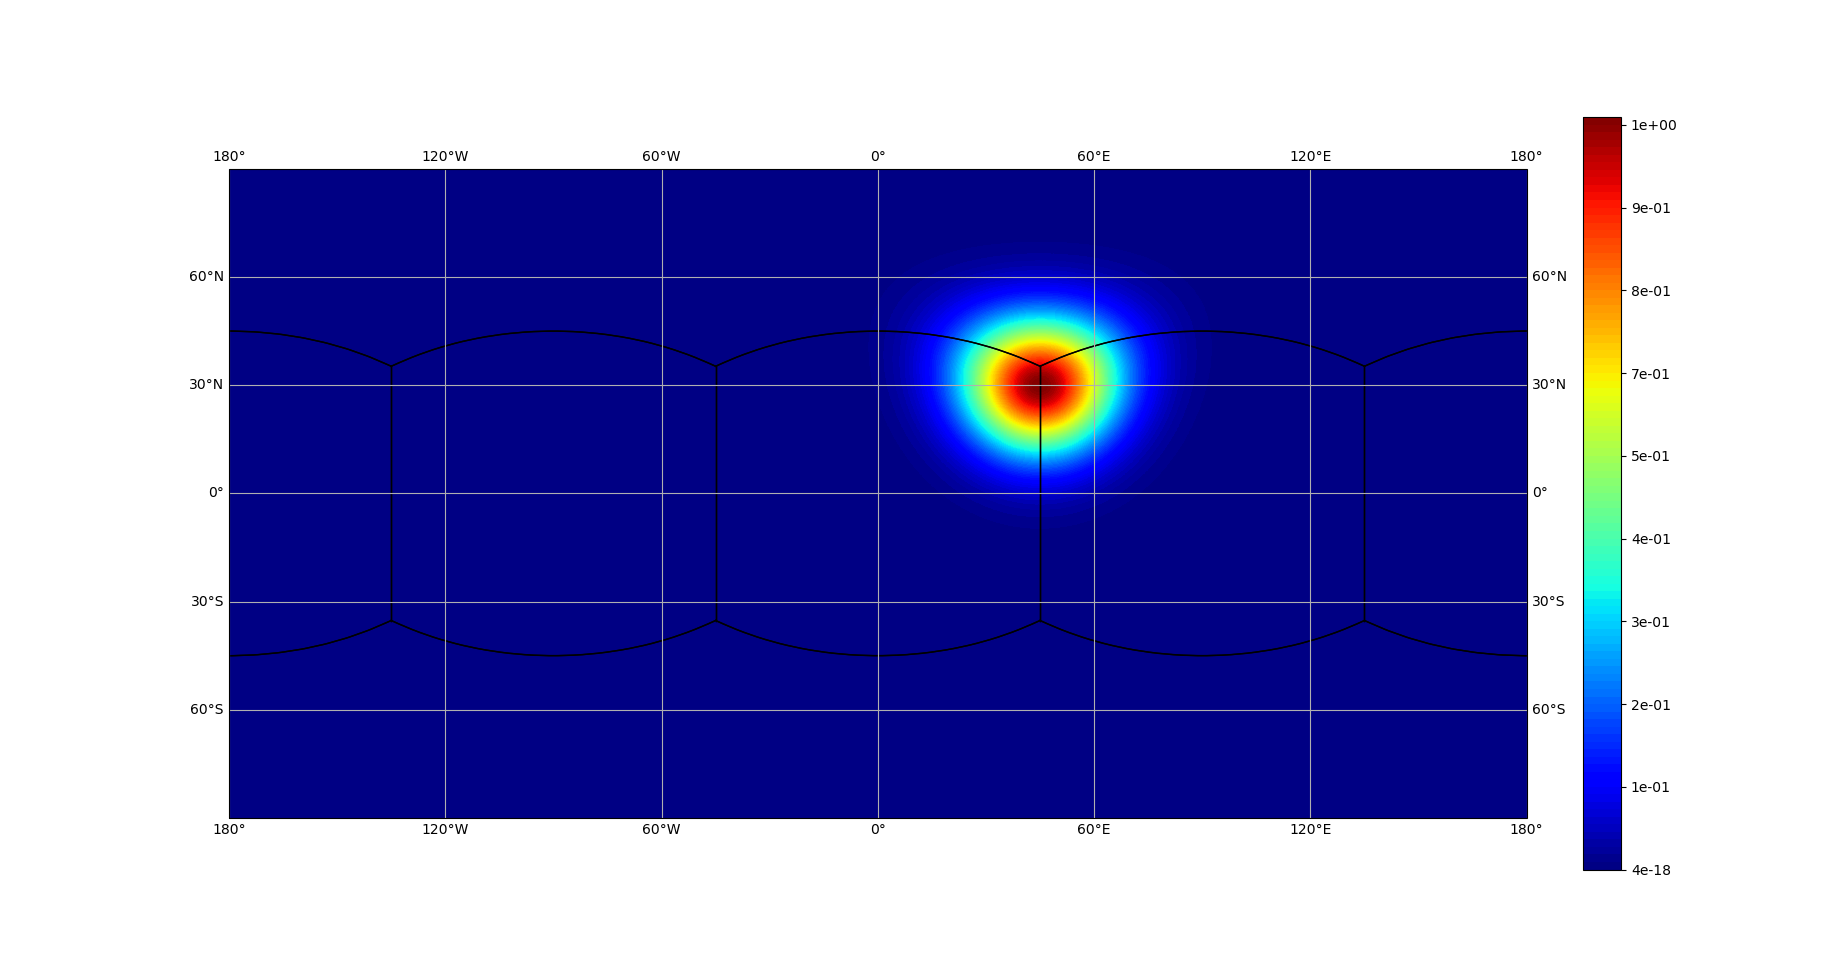
\includegraphics[width=0.9\linewidth]{gnomonic_equidistant_1024_interp_q_ic_1_mercator}
	\caption{Gaussian defined by Equation \eqref{chp4-ic1}.}
	\label{chp4-cs-ic1}
\end{figure}

We shall also consider the following trigonometric function, which is the divergence of a velocity field,
as in \citet{peixoto:13} in our tests:
\begin{align}
	\label{chp4-ic2}
	\begin{split}
	q(\lambda, \phi) = \frac{1}{\cos(\phi)}\bigg(-2\cos^3(\phi) \sin(\lambda) \cos(\lambda)
	+16\sin^2(\lambda)\cos(\lambda)\cos^3(\phi)\sin(\phi)\bigg),
	\end{split}
\end{align}
whose graph is depicted in Figure \ref{chp4-cs-ic2}.
\begin{figure}[!htb]
	\centering
	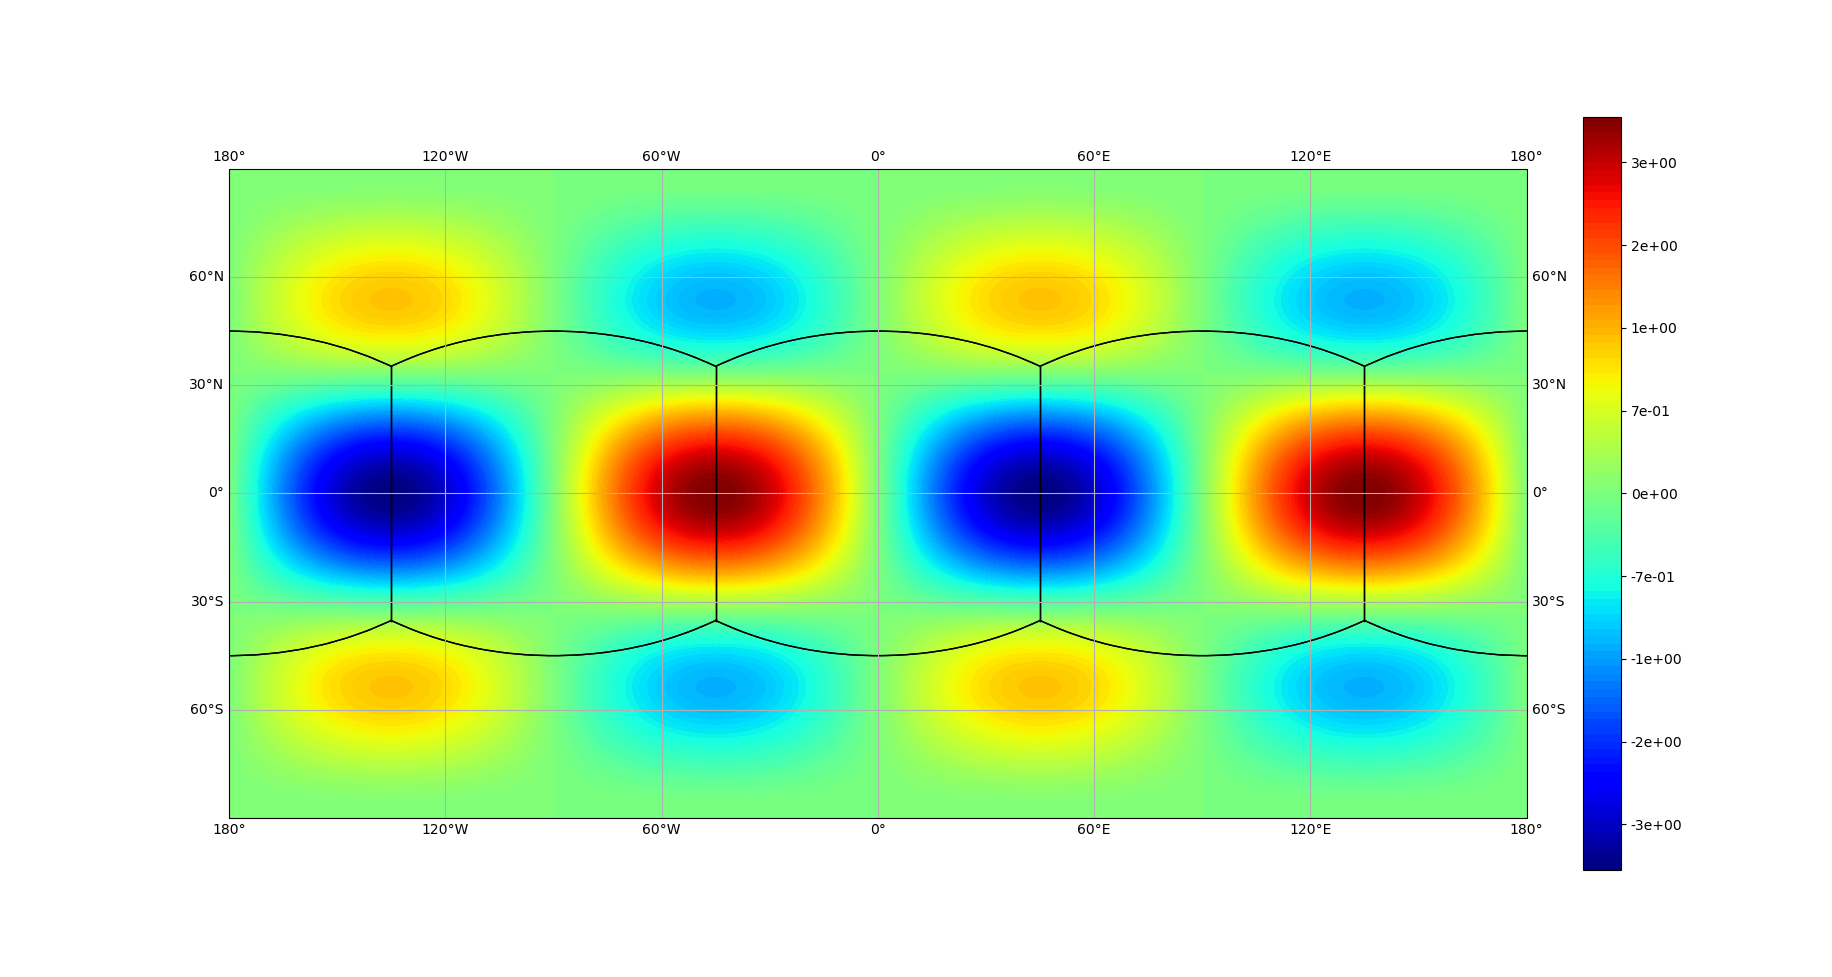
\includegraphics[width=1\linewidth]{gnomonic_equidistant_1024_interp_q_ic_2_mercator}
	\caption{Trigonometric function defined by Equation \eqref{chp4-ic2}.}
	\label{chp4-cs-ic2}
\end{figure}

We are going to consider the relative error in the maximum norm and the convergence rate 
at the host cell positions defined analogously as in Section \ref{sec-ds-exp}. 
We also consider values os $N$ given by $2^k$, for $k=4, \cdots, 10$, in order to compute the error and convergence rate.
\begin{figure}[!htb]
	\centering
	\begin{subfigure}{0.45\textwidth}
		\centering
		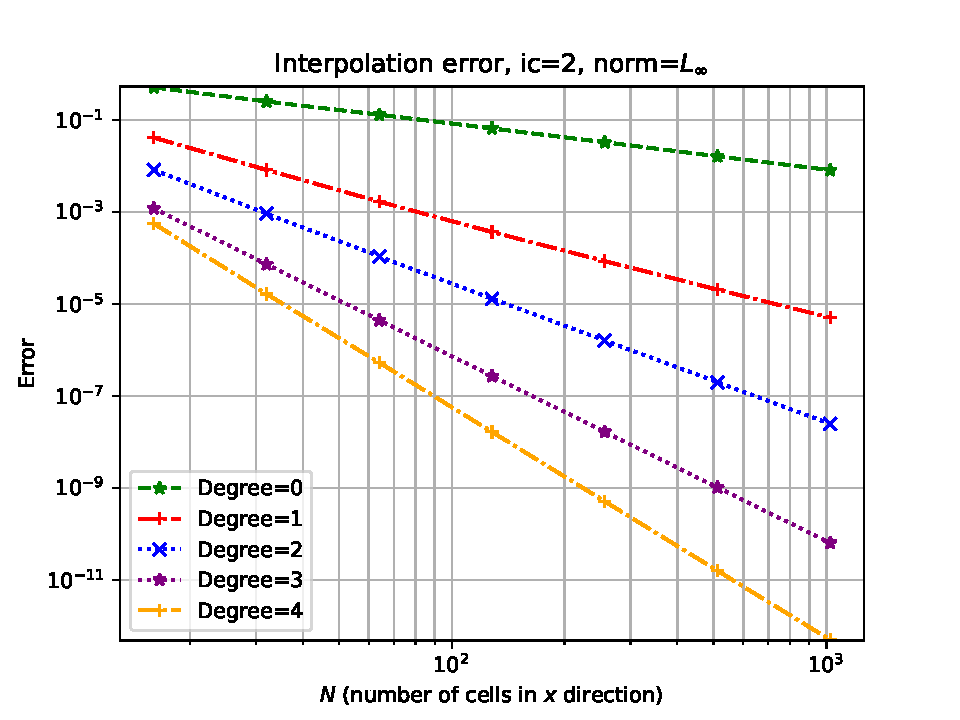
\includegraphics[width=1\linewidth]{cs_interp_ic2_normlinf_errors}
		\caption{Error.\label{chp4-exp1-error}}
	\end{subfigure}
	\begin{subfigure}{0.45\textwidth}
		\centering
		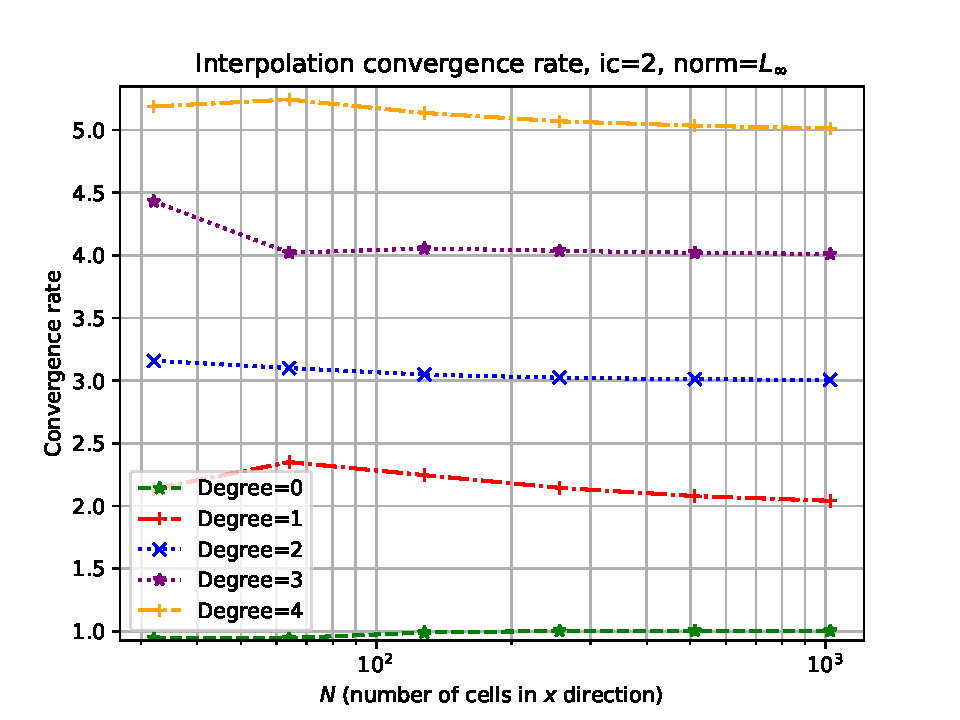
\includegraphics[width=1\linewidth]{cs_interp_ic2_normlinf_convergence_rate}
		\caption{Convergence rate.\label{chp4-exp1-CR}}
	\end{subfigure}
	\caption{Relative error convergence (a) and convergence rate (b) for the ghost cell interpolation process for different
		polynomial degrees, using the Gaussian function given by Equation \eqref{chp4-ic1}.\label{chp4-exp1}}
\end{figure}

\begin{figure}[!htb]
	\centering
	\begin{subfigure}{0.45\textwidth}
		\centering
		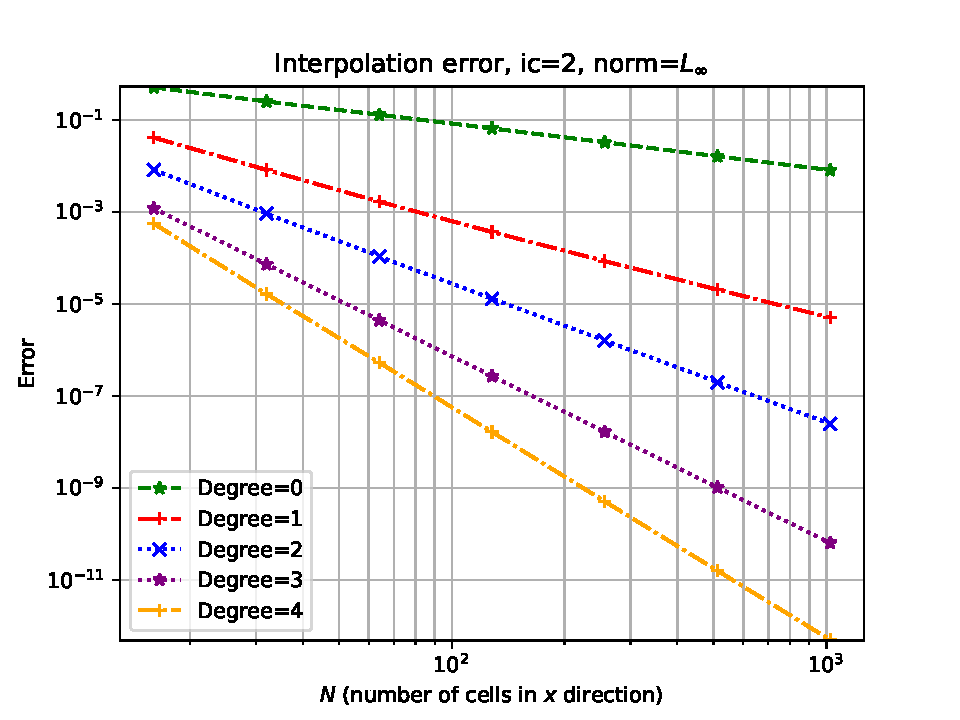
\includegraphics[width=1\linewidth]{cs_interp_ic2_normlinf_errors}
		\caption{Error.\label{chp4-exp2-error}}
	\end{subfigure}
	\begin{subfigure}{0.45\textwidth}
		\centering
		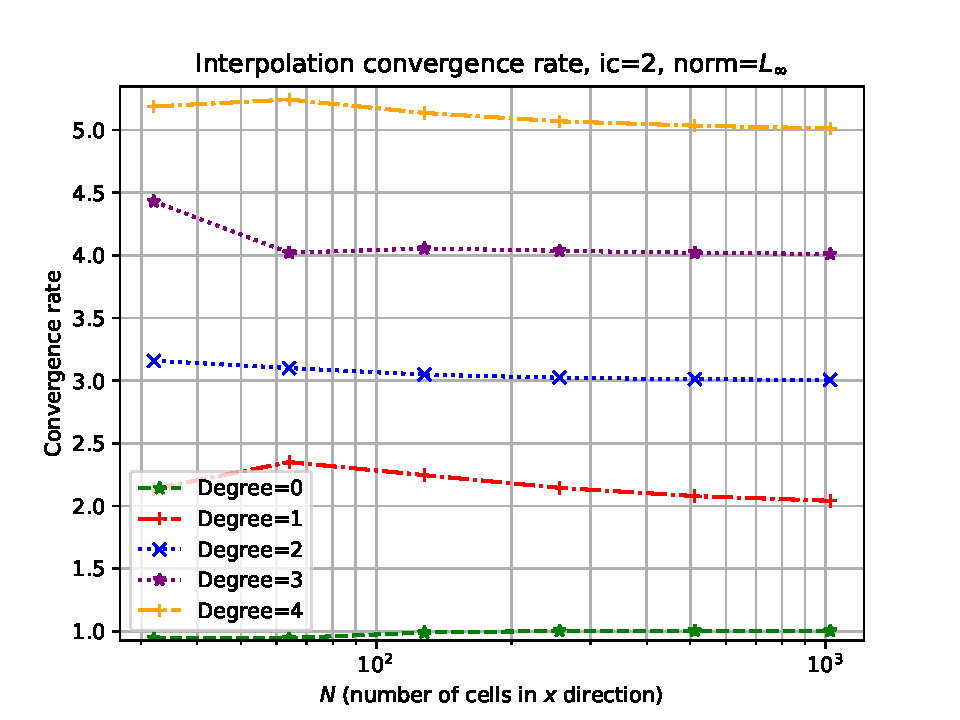
\includegraphics[width=1\linewidth]{cs_interp_ic2_normlinf_convergence_rate}
		\caption{Convergence rate.\label{chp4-exp2-CR}}
	\end{subfigure}
	\caption{As Figure \ref{chp4-exp1} but using the trigonometric function given by Equation \eqref{chp4-ic2}.\label{chp4-exp2}}
\end{figure}
\break
In Figures \ref{chp4-exp1} and \ref{chp4-exp2} we show the errors and convergence rate for the functions from Equations \eqref{chp4-ic1} and \eqref{chp4-ic2},
respectively, considering polynomials of degrees from 0 up to 4. As both graphs show, we were able to achieve the expected order of convergence.
Next, we shall use the ghost cell interpolation when computing the stencils from PPM edge reconstructions presented in Chapter \ref{chp-1d-fv}
in each direction of a panel and also compare the results obtained with extrapolation.

\subsection{Edges reconstruction}
\label{cs-recon}
Let denote a control volume of the cubed-sphere by $\Omega_{ijp}$, that is:
\begin{equation*}
	\Omega_{ijp} = \Phi_p([x_{i-\frac{1}{2}}, x_{i+\frac{1}{2}}] \times [y_{j-\frac{1}{2}}, y_{j+\frac{1}{2}}]),
	\quad 1 \leq i, j \leq N, \quad 1 \leq p \leq 6.
\end{equation*}
We define the average values of a function $q$ with the aid of the metric tensor $g(x,y)$ (Equation \ref{metrictensor-cs-equiangular}):
\begin{equation*}
	Q_{ijp} = \frac{1}{|\Omega_{ijp}|}\int_{x_{i-\frac{1}{2}}}^{x_{i+\frac{1}{2}}}
	\int_{y_{j-\frac{1}{2}}}^{y_{j+\frac{1}{2}}}  q(x,y;p) \sqrt{g(x,y)}\,dx \,dy,
\end{equation*}
where $|\Omega_{ijp}|$ is the control volume area given by:
\begin{equation*}
	|\Omega_{ijp}| = \int_{x_{i-\frac{1}{2}}}^{x_{i+\frac{1}{2}}} \int_{y_{j-\frac{1}{2}}}^{y_{j+\frac{1}{2}}}\sqrt{g(x,y)} \,dx \,dy.
\end{equation*}
Similar to Proposition \ref{prop-bound-centroid-2d}, we may approximate the average value using the centroid value, that is
\begin{equation*}
	Q_{ijp} - q_{ijp} = O(\Delta x ^2), 
\end{equation*}
where $q_{ijp} = q(x_i,y_j; p)$, recalling that on the cubed-sphere we always assume $\Delta x = \Delta y$.
In this work, we shall always approximate the average values since our schemes are expected to be at most second-order,
this approximation does not deteriorate the convergence order.

Let us consider the following problem: given the values $q_{ijp}$ we wish to find approximations of 
the function $q$ at the control volume edge midpoints denoted by
$q^{L,x}_{ijp}  \approx q_{{i-\frac{1}{2}},j,p}$,
$q^{R,x}_{ijp}  \approx q_{{i+\frac{1}{2}},j,p}$,
$q^{L,y}_{ijp}  \approx q_{i,{j-\frac{1}{2}},p}$,
$q^{R,y}_{ijp}  \approx q_{i,{j+\frac{1}{2}},p}$, where we also using the notations
$q_{{i+\frac{1}{2}},j,p}  \approx q(x_{i+\frac{1}{2}},y_j; p)$,
$q_{i,{j+\frac{1}{2}},p}  \approx q(x_i,y_{j+\frac{1}{2}}; p)$.
These points are illustrated in Figure \ref{csgrid-rpoints} for panel 1.
\begin{figure}[!htb]
	\centering
	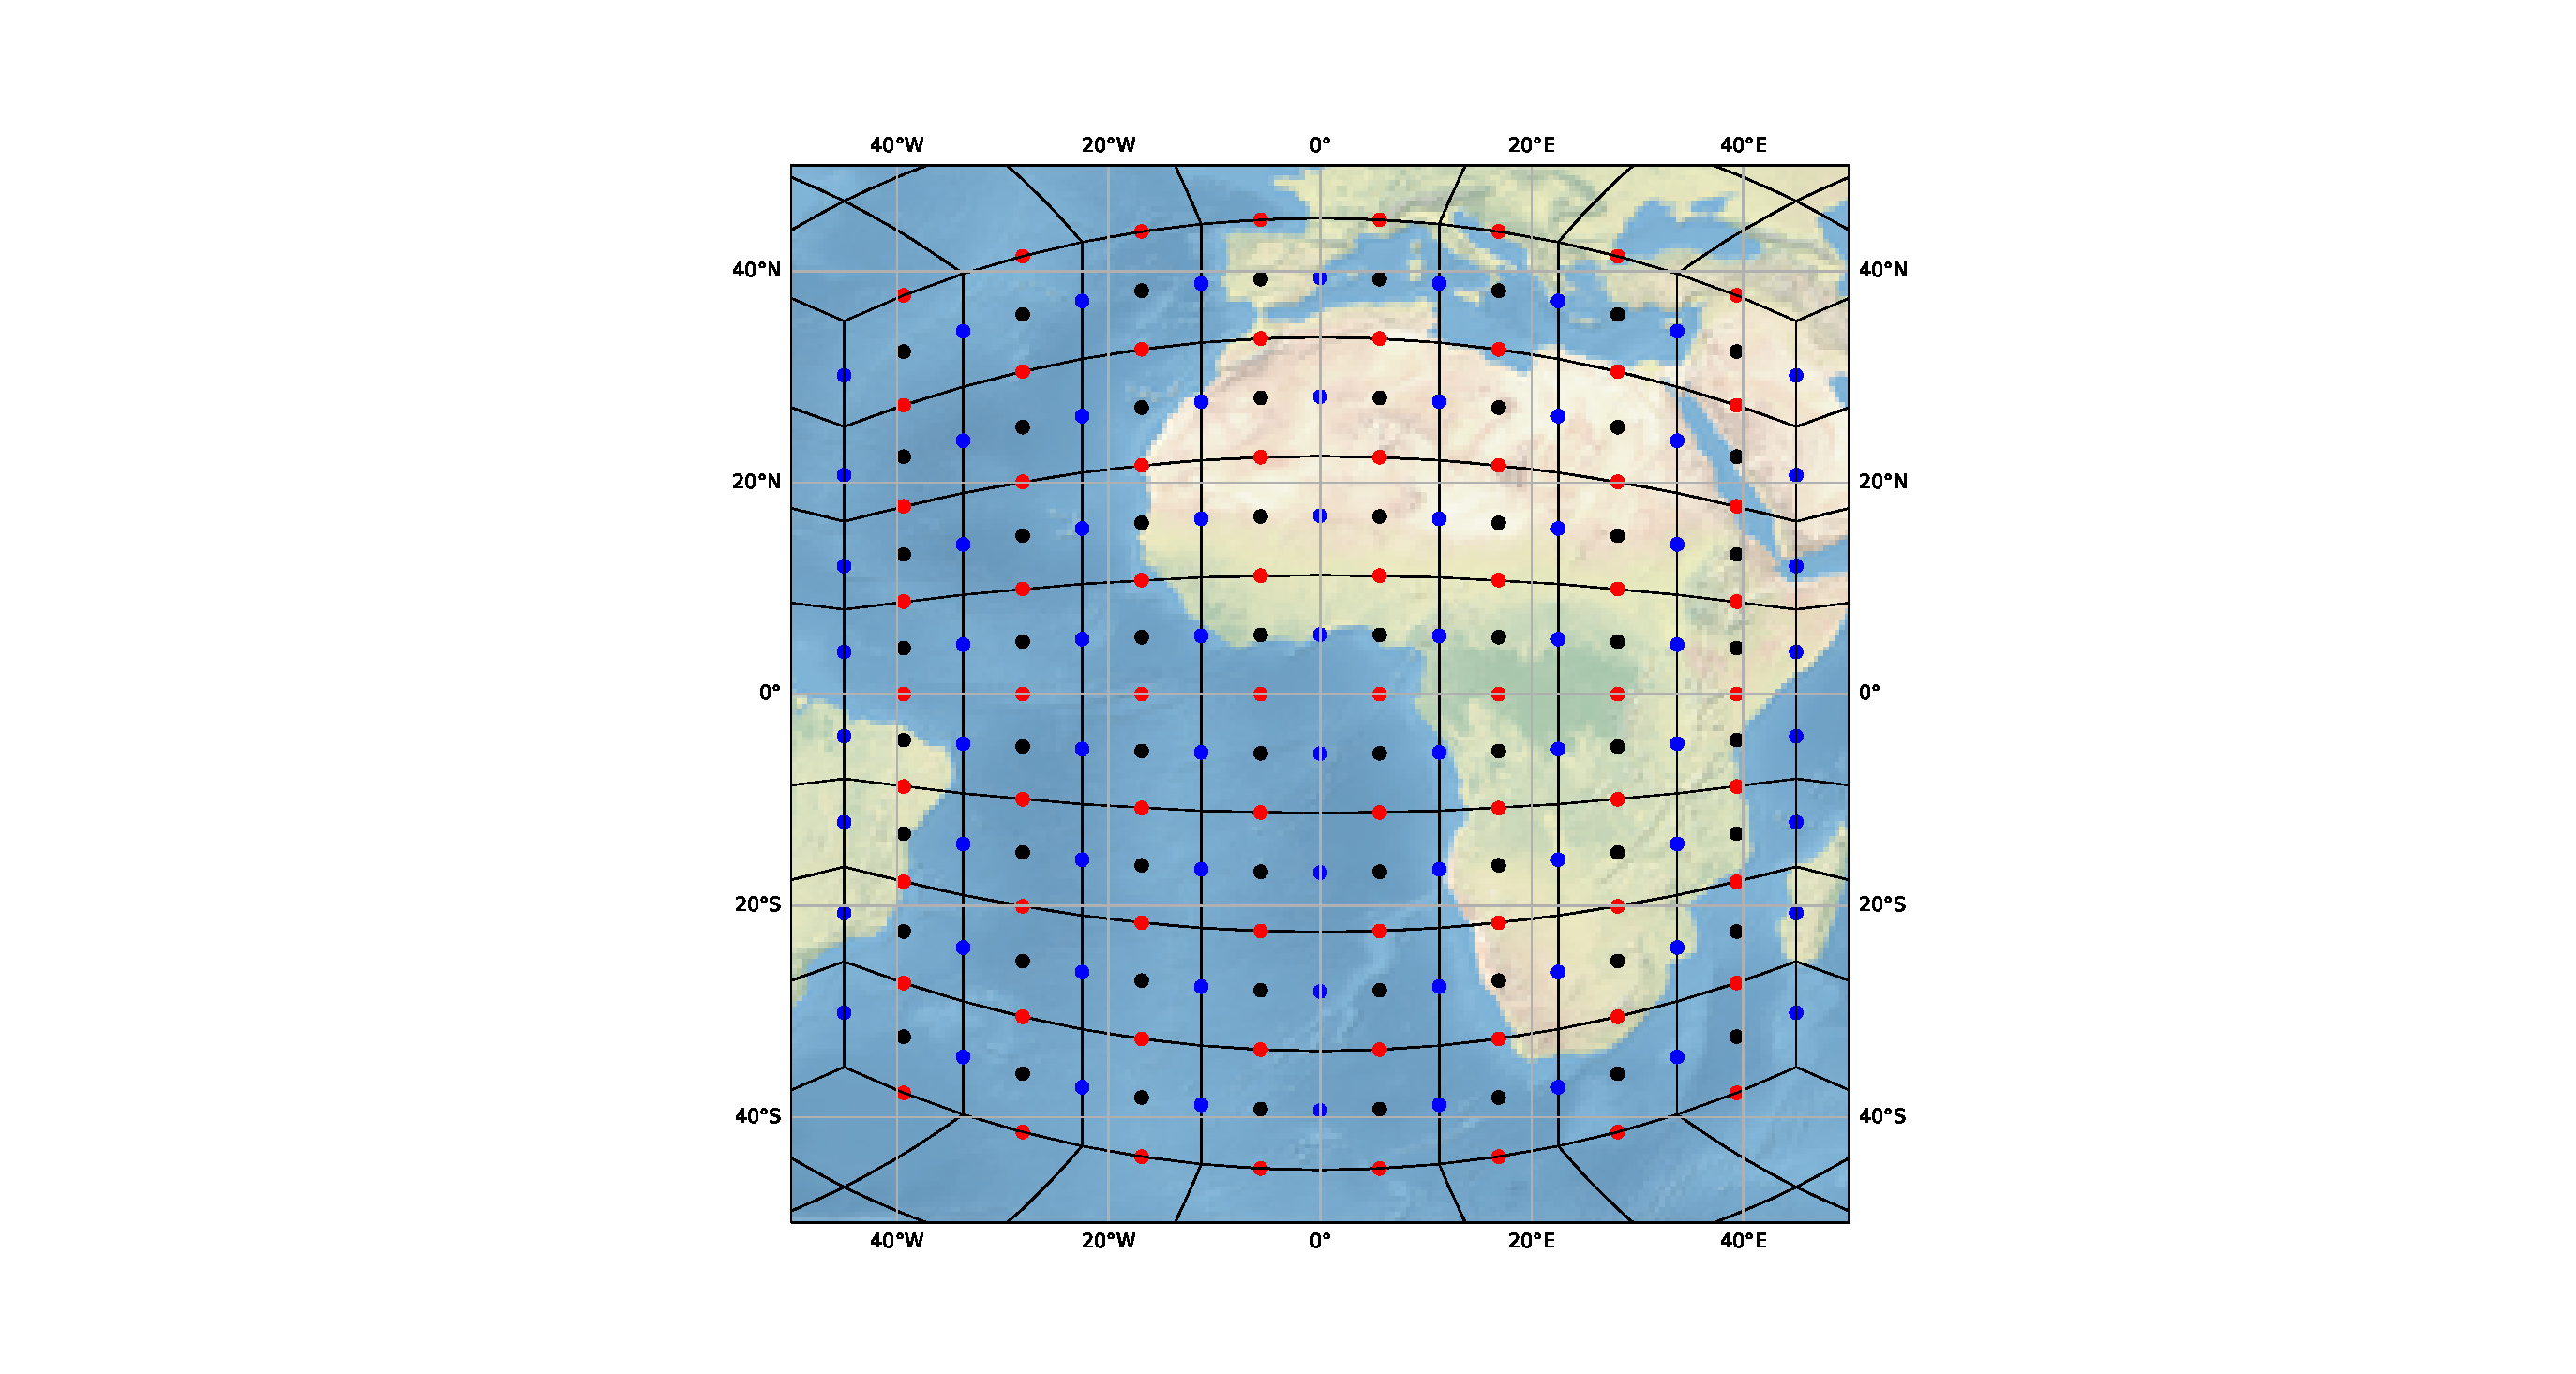
\includegraphics[width=1\linewidth]{gnomonic_equiangular_8_mercator_2}
	\caption{The reconstruction problem on the cubed-sphere panel 1: we are given the centroid values of a function (black circles)
		and we wish to estimate these values at the edges midpoints in the $x$ direction (blue circles) and $y$ direction (red circles).
		This figure uses an equiangular cubed-sphere with $N=8$.} \label{csgrid-rpoints}
\end{figure}

We can estimate the desired values using the one-dimensional reconstruction schemes from Sections \ref{chp2-sec-recon} and \ref{chp2-sec-mono}
by performing the PPM reconstruction in the $x$ and $y$ directions independently. Notice that all the schemes from 
Sections \ref{chp2-sec-recon} and \ref{chp2-sec-mono} are expected to be second-order accurate due to centroid point approximation.
The major difference here is that when we compute the stencil near the cube edges. Unlikely the previous chapters where we
assumed periodic boundary conditions, the boundary conditions are related to the adjacent panel.
One to overcome this problem is just to add ghost cell layers and use the process described in Section \ref{cs-interp}, hence
all the stencils may be computed. This approach shall be referred to as \textbf{ET-1} (ET stands for edge treatment).
Observe that the points that lie on a cube edge are computed twice, where each calculation uses one adjacent panel per time.
One possible way to uniquely define this value while preserving the order is
to average the two values obtained by the adjacent panels. This scheme is named \textbf{ET-2}.

An approach that avoids the use of ghost has been developed by \citet{putman:2007} using 
extrapolation at the cells surrounding to the cube edge.
We are going to describe this scheme that we shall name \textbf{ET-3}. This scheme uses the extrapolation:
\begin{align*}
	q^{L,x}_{1,j,p} &= \frac{1}{2}\bigg(3Q_{1,j,p} - Q_{2,j,p}\bigg),\\
	q^{R,x}_{N,j,p} &= \frac{1}{2}\bigg(3Q_{N,j,p} - Q_{N-1,j,p}\bigg),\\
	q^{L,y}_{i,1,p} &= \frac{1}{2}\bigg(3Q_{i,1,p} - Q_{i,2,p}\bigg),\\
	q^{R,y}_{i,N,p} &= \frac{1}{2}\bigg(3Q_{i,N,p} - Q_{i,N-1,p}\bigg),\\
\end{align*}
at the points that are located on the cube edges. The other edge values are estimated as:
\begin{align*}
	q^{R,x}_{1,j,p} &= \frac{1}{14}\bigg(3Q_{1,j,p} + 11Q_{2,j,p} - 2(Q_{3,j,p} - Q_{1,j,p})\bigg),\\
	q^{L,x}_{2,j,p} &= q^{R,x}_{1,j,p},\\
	q^{L,x}_{N,j,p} &= \frac{1}{14}\bigg(3Q_{N,j,p} + 11Q_{N-1,j,p} - 2(Q_{N-2,j,p} - Q_{N,j,p})\bigg),\\
	q^{R,x}_{N-1,j,p} &= q^{L,x}_{N,j,p},\\
\end{align*}
in the $x$ direction and in the $y$ direction we use the formulas
\begin{align*}
	q^{R,y}_{i,1,p} &= \frac{1}{14}\bigg(3Q_{i,1,p} + 11Q_{i,2,p} - 2(Q_{i,3,p} - Q_{i,1,p})\bigg),\\
	q^{L,y}_{i,2,p} &= q^{R,x}_{i,1,p},\\
	q^{L,y}_{i,N,p} &= \frac{1}{14}\bigg(3Q_{i,N,p} + 11Q_{i,N-1,p} - 2(Q_{i,N-2,p} - Q_{i,N,p})\bigg),\\
	q^{R,y}_{i,N-1,p} &= q^{L,y}_{i,N,p}.\\
\end{align*}
Again, we can average to values at the cube edges, which leads to the scheme named \textbf{ET-4}.
We are going to use the trigonometric (Equation \eqref{chp4-ic1}) functions
as before on the unit sphere to compare the schemes ET-1, ET-2, ET-3 and ET-4. The scheme ET-1 and ET-2
uses cubic polynomials.
We going to introduce the relative errors:
\begin{align*}
	e_{{i-\frac{1}{2}},j,p} &= (|q_{{i-\frac{1}{2}},j,p} - q^{L,x}_{ijp}|)/|q_{{i-\frac{1}{2}},j,p}|,\\
	e_{{i+\frac{1}{2}},j,p} &= (|q_{{i+\frac{1}{2}},j,p} - q^{R,x}_{ijp}|)/|q_{{i+\frac{1}{2}},j,p}|,\\
	e_{i,{j-\frac{1}{2}},p} &= (|q_{i,{j-\frac{1}{2}},p} - q^{L,y}_{ijp}|)/|q_{i,{j-\frac{1}{2}},p}|,\\
	e_{i,{j+\frac{1}{2}},p} &= (|q_{i,{j+\frac{1}{2}},p} - q^{R,y}_{ijp}|)/|q_{i,{j+\frac{1}{2}},p}|,\\
	e_{ijp} &= \max\{e_{{i-\frac{1}{2}},j,p}, e_{{i+\frac{1}{2}},j,p} , e_{i,{j-\frac{1}{2}},p}, e_{i,{j+\frac{1}{2}},p} \},\\
	E &= \max \{e_{ijp}\}.
\end{align*}
We are going to compute $E$ for different values of $N$ as in the numerical experiments of Section \ref{cs-interp}.
\begin{figure}[!htb]
	\centering
	\begin{subfigure}{0.45\textwidth}
		\centering
		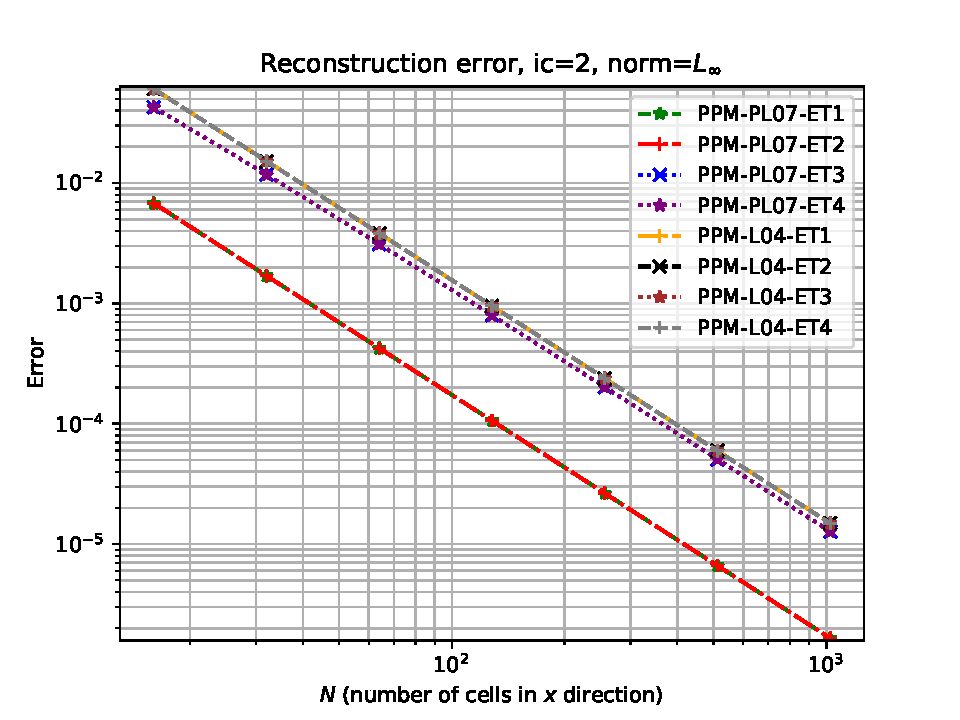
\includegraphics[width=1\linewidth]{cs_recon_ic2_normlinf_parabola_errors}
		\caption{Error.\label{chp4-exp3-error}}
	\end{subfigure}
	\begin{subfigure}{0.45\textwidth}
		\centering
		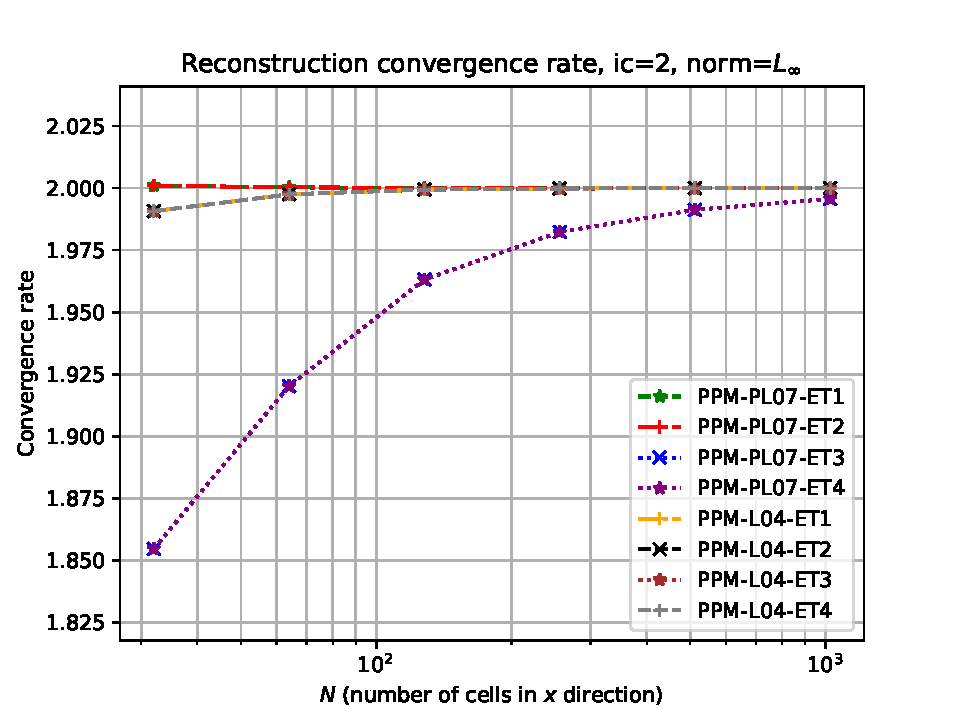
\includegraphics[width=1\linewidth]{cs_recon_ic2_normlinf_convergence_rate}
		\caption{Convergence rate.\label{chp4-exp3-CR}}
	\end{subfigure}
	\caption{Relative error convergence (a) and convergence rate (b) for the reconstruction problem for different
	edge treatments (ET), using the trigonometric function given by Equation \eqref{chp4-ic2}.\label{chp4-exp3}}
\end{figure}

In Figure \ref{chp4-exp3} we show the errors and the convergence rate using the PPM-PLO07 and PPM-L04 reconstruction schemes.
We can observe that all the schemes converge to zero with second-order.
Besides that, the scheme ET-1 and ET-2 produce essentially the same error, and so are the schemes ET-3 and ET-4.
The difference between the ghost cell interpolation-based schemes and the extrapolation-based schemes
may be observed in Figure \ref{chp4-exp4} and Figure \ref{chp4-exp5}, for the  PPM-PL07 and PPM-L04 reconstruction schemes,
respectively.
We notice that the cube edges appear on the error graph when we use the ET-4 scheme. This is an example of grid imprinting.
Although all schemes are second-order, the ghost cell interpolation-based schemes do seem to produce grid imprinting
in the reconstruction problem.
The graphs of ET1 are very similar to the graph of ET-2 and the graphs of ET-3 are very similar to the graph of ET4 (not shown).
\newpage
\begin{figure}[!htb]
	\centering
	\begin{subfigure}{0.49\textwidth}
		\centering
		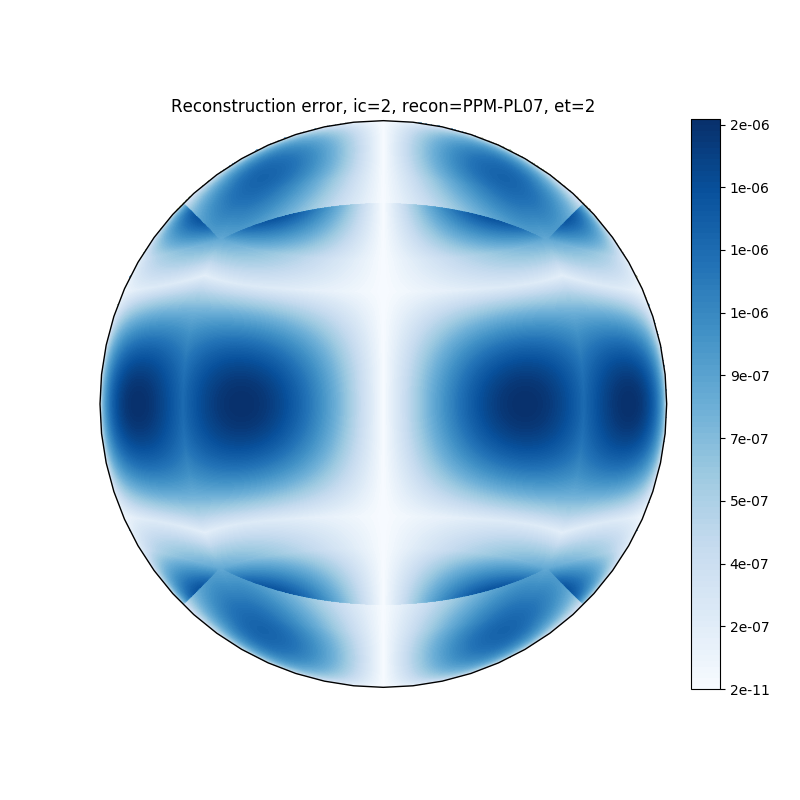
\includegraphics[width=1\linewidth]{gnomonic_equiangular_1024_recon_q_ic_2_reconPPM-PL07_et2_sphere}
		\caption{ET-2.\label{chp4-exp4-a}}
	\end{subfigure}
	\begin{subfigure}{0.49\textwidth}
		\centering
		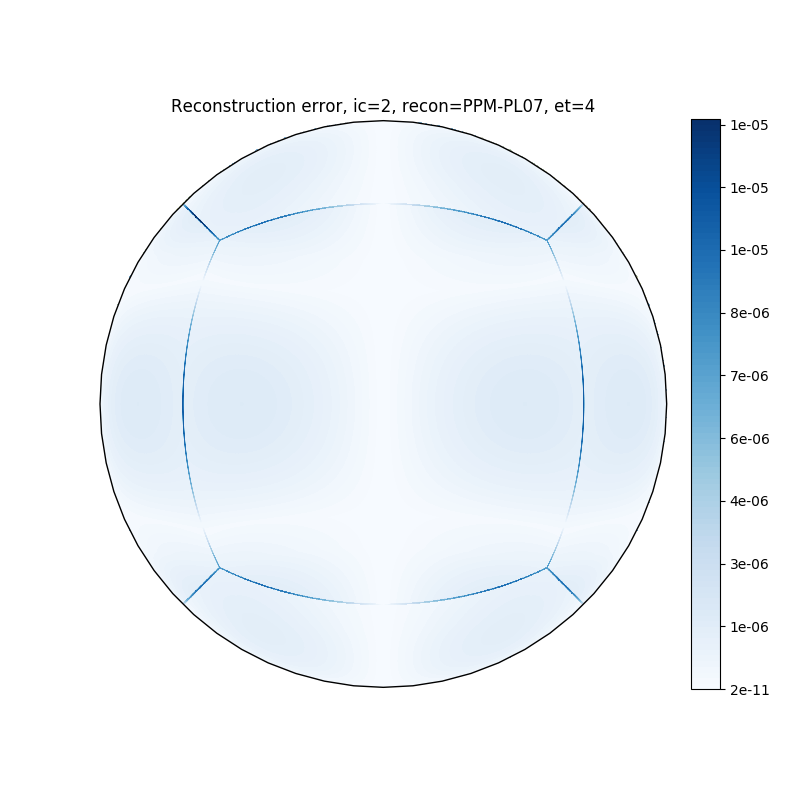
\includegraphics[width=1\linewidth]{gnomonic_equiangular_1024_recon_q_ic_2_reconPPM-PL07_et4_sphere}
		\caption{ET-4.\label{chp4-exp4-b}}
	\end{subfigure}
	\caption{Error for the edge midpoint values considering the trigonometric function (Equation \eqref{chp4-ic2})
		with edges treatment schemes ET-2 (a) and ET-4 (b) for the cubed-sphere with $N=1024$ using the reconstruction PPM-PL07.\label{chp4-exp4}}
\end{figure}

\begin{figure}[!htb]
	\centering
	\begin{subfigure}{0.49\textwidth}
		\centering
		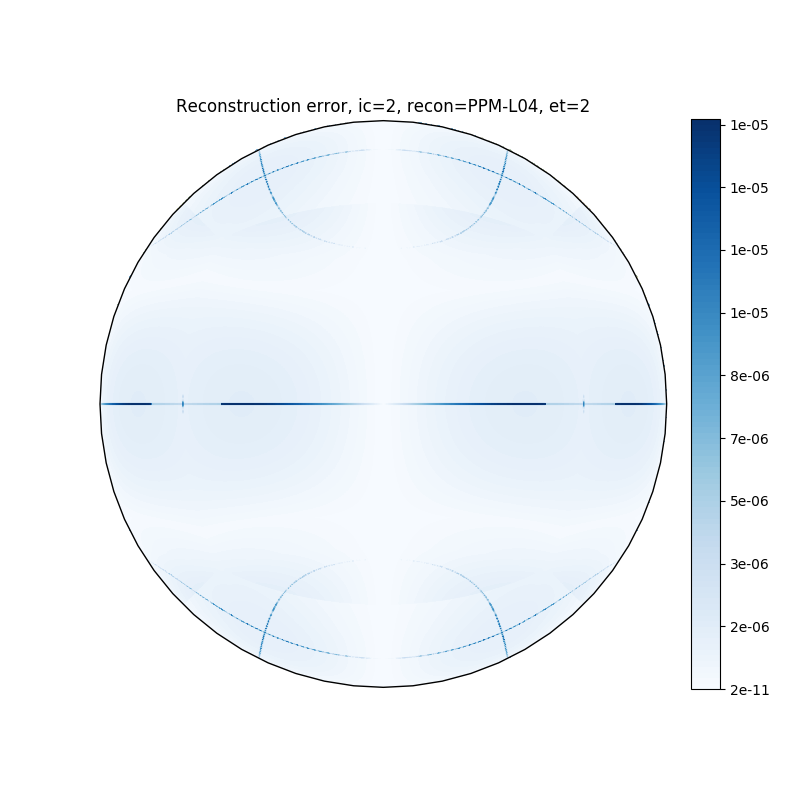
\includegraphics[width=1\linewidth]{gnomonic_equiangular_1024_recon_q_ic_2_reconPPM-L04_et2_sphere}
		\caption{ET-2.\label{chp4-exp5-a}}
	\end{subfigure}
	\begin{subfigure}{0.49\textwidth}
		\centering
		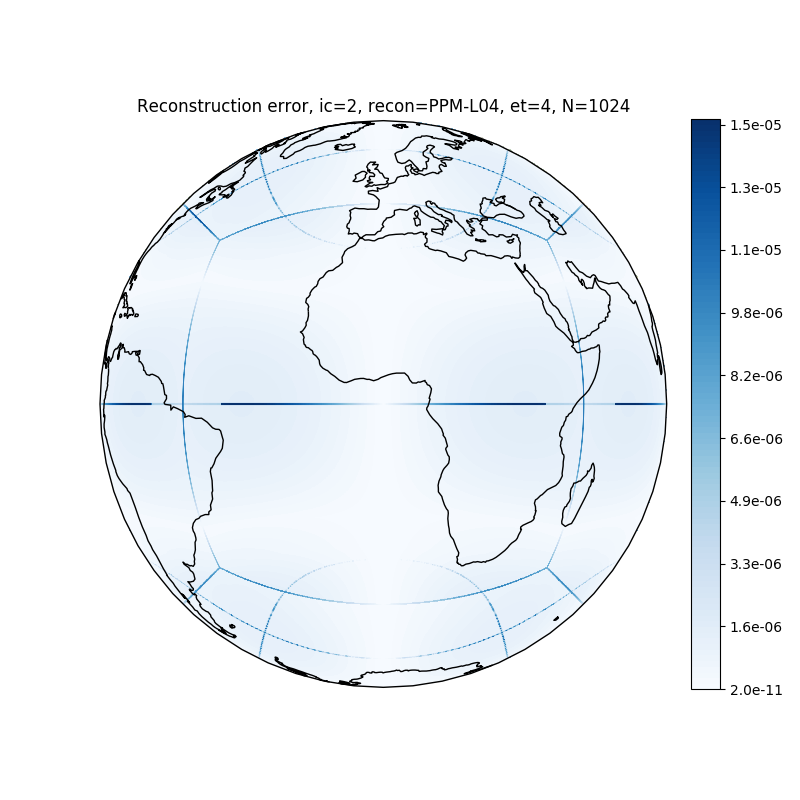
\includegraphics[width=1\linewidth]{gnomonic_equiangular_1024_recon_q_ic_2_reconPPM-L04_et4_sphere}
		\caption{ET-4.\label{chp4-exp5-b}}
	\end{subfigure}
	\caption{As Figure in \ref{chp4-exp4} but using the PPM-L04 scheme.\label{chp4-exp5}}
\end{figure}